\section{Asynchronous Advantage Actor Critic}
\label{sec:A3C}
The newest breakthrough in RL is the \textit{Asynchronous Advantage Actor Critic} (A3C) approach, and therefore it was chosen to be studied and implemented onto the idea of driver-less cars. In order to achieve a similar environment as the one of a car, and also to be able to get the necessary data easier, a car simulator was chosen for the project. Among the existing car simulators encountered in the different online sources, and after analyzing the DDPG implementation on The Open Racing Car Simulator (TORCS) \cite{DDPG_Torcs}, the project settled for this car simulator as well.

The project was mainly inspired from the article \cite{DBLP:journals/corr/MnihBMGLHSK16} summarized in the section \ref{AsyncMeths}, and also from the recent implementation of the A3C into the Doom game elaborated on in \cite{A3CDoom}.

The idea behind the A3C is very much around the same \textit{actor-critic} approach described in the section \ref{PolicyGradMeths} and in the Figure \ref{fig:Actor_critic_architecture}, that, more accurately, is founded on the presence of both the value function approximator, $\theta_{v}$ and the bootstrapping policy estimator, $\theta$. An additional feature of the actor-critic method is the \textit{asynchronous} part. Instead of having a single agent training on the GPU as in the example of the DDPG project elaborated in the previous section, multiple agents are instantiated for training on different CPU threads simultaneously, and, unlike in the DDPG where there are two different networks, in the A3C the agents share a global network, which is updated as the agents advance. Another new feature of the A3C is the \textit{advantage} element, which is just a mathematical way of expressing how much better some actions ended up to be, and where the estimation should be improved. The update performed by the A3C is of the form $\nabla_{\theta'}\textup{log}\pi(a|s,\theta')A(s,a,\theta,\theta_{v})$, and the formula for the advantage is $\sum_{i=0}^{k-1}\gamma^{i}r_{t+i}+\gamma^kV(s_{t+k},\theta_{v})-V(s_{t},\theta_{v})$, which are both taken from the article \cite{DBLP:journals/corr/MnihBMGLHSK16}. The update formula changes slightly after including the entropy factor in the policy in order to encourage exploration and avoid convergence to an earlier suboptimal solution. The detailed A3C algorithm taken from \cite{DBLP:journals/corr/MnihBMGLHSK16} is listed below:
\begin{algorithm}[H]
	\caption{Asynchronous advantage actor-critic - pseudocode for each actor-learner thread.}
	\label{algo:A3C}
	\begin{algorithmic}
		\State \textit{//Assume global shared parameter vectors $\theta$ and $\theta_{v}$ and counter $T=0$}
		\State \textit{//Assume thread-specific parameter vectors $\theta'$ and $\theta_{v}'$}
		\State Initialize thread step counter $t\leftarrow1$
		\Repeat
		\State Reset gradients: $d\theta\leftarrow 0$ and $d\theta_{v}\leftarrow0$
		\State Synchronize thread-specific parameters $\theta'=\theta$ and $\theta_{v}'=\theta_{v}$
		\State $t_{start}=t$
		\State Get state $s_{t}$
		\Repeat
		\State Perform action $a_{t}$ according to policy $\pi(a_{t}|s_{t}, \theta')$
		\State Receive reward $r_{t}$ and new state $s_{t+1}$
		\State $t\leftarrow t+1$
		\State $T\leftarrow T+1$
		\Until terminal \textbf{or} $t-t_{start}==t_{max}$
		\If {$s_{t}$ is terminal}
		\State $R=0$
		\Else 
		\State $R=V(s_{t},\theta_{v}')$ \textit{//bootstrap from last state }
		\EndIf
		\For {$i \in \left \{ t-1,...,t_{start} \right \}$}
		\State $R\leftarrow r_{i}+\gamma R$
		\State Accumulate gradients wrt $\theta'$:
		\State $d\theta\leftarrow d\theta+\nabla_{\theta'}\textup{log}\pi(a_{i}|s_{i},\theta')(R-V(s_{i},\theta_{v}'))$
		\State Accumulate gradients wrt $\theta_{v}'$:
		\State $d\theta_{v}\leftarrow d\theta_{v} + \partial (R-V(s_{i},\theta_{v}'))^2/ \partial\theta_{v}'$
		\EndFor
		\State Perform asynchronous update of $\theta$ using $d\theta$ and of $\theta_{v}$ using $d\theta_{v}$
		\Until $T>T_{max}$
	\end{algorithmic}
\end{algorithm}

\subsection{Project Description}
The A3C implementation into the Doom game uses images generated by the vizDoom environment as input data for the well known nonlinear function approximation solution method - ANN. The images become the \textit{states} of the RL problem based on which the AI agent learns to shoot the opponents. The vizDoom environment has a \textit{reward} function predefined, which is triggered when the agent deploys an action in the environment. As the given implementation was made for the \textit{discrete actions space}, the estimated policy or the \textit{actor} provides the probabilities of taking each action in a specific state, and so, in each state, the action with the maximal probability is chosen to be pursued. The \textit{critic}, on the other hand, estimates a state-value function for the existing policy and it is used in the composition of the loss function, which represents the performance measure or the \textit{objective function} of the RL problem.

The A3C project developed for the TORCS environment has the same principles as the A3C Doom. It also uses images as the input states into a deep ANN structure and the mathematical model of the problem is similar. The TORCS environment is more flexible and that is an advantage as it offers more freedom for changing things and get better results. For example, it is easier to change the reward function and perform action manipulations, and this will be further explained and illustrated in the next chapter. Another additional implementation is the \textit{continuous} actions space, which is slightly different than the \textit{discrete} actions space implementation; nevertheless, they were both preserved in the project for analysis purposes. 

\subsection{ANN Structure}\label{ANNstructure}
The structure of the deep ANN will offer more insight on how the program works. Therefore, the overall structure of the ANN of the A3C TORCS project is presented in the following figure:
\begin{figure}[H]
	\centering
	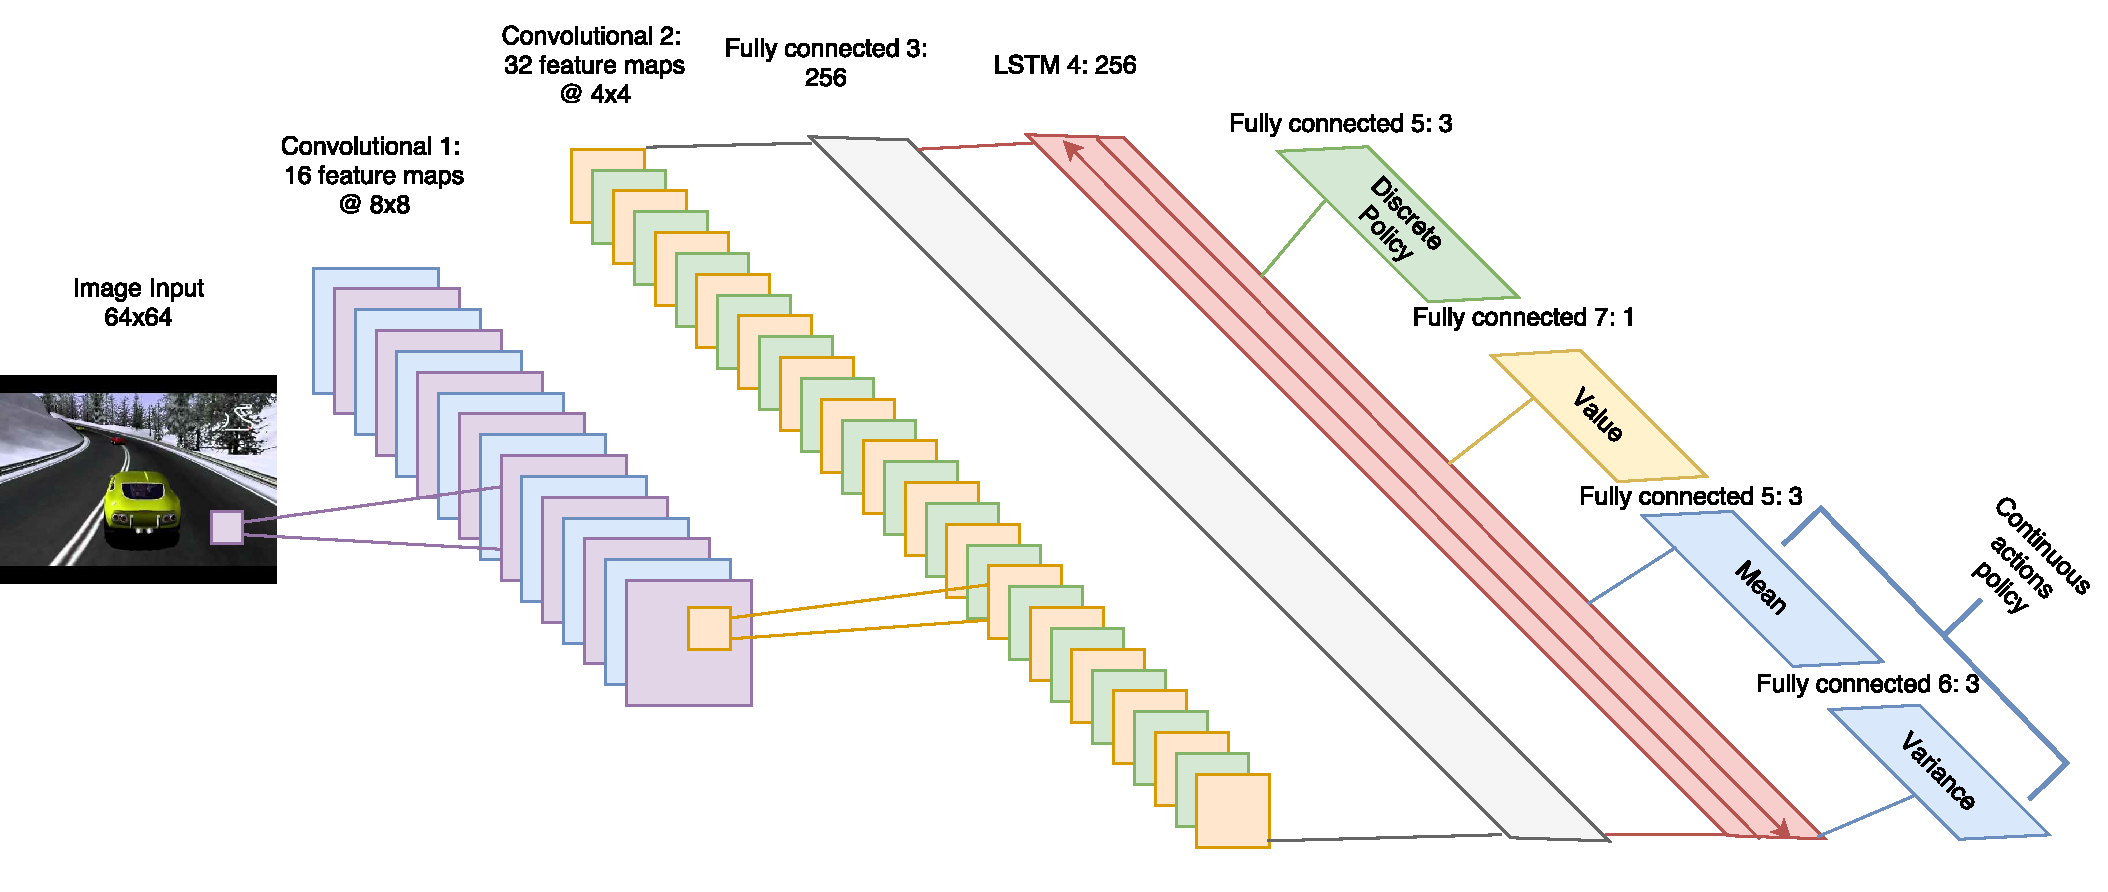
\includegraphics[width=1.25\textwidth]{Figures/A3CTorcs}
	\caption{The ANN structure of the A3C implementation into Torcs}
	\label{A3CTorcs}
\end{figure}
The gray-scale image of size 64x64 comes into the ANN as input and goes through the first layer of ANN - a convolutional layer that outputs 16 feature maps of sizes 8x8 each. Next, these are again passed through another convolutional layer that outputs 32 feature maps of size 4x4 each, while taking care of spatial correlations. Then the output is flattened with a fully connected layer and passed to a recurrent layer - basic LSTM, that takes care of the temporal dependencies. Finally, the output of the LSTM layer can be used for the last layers of the ANN. The value function is linearly estimated, while the discrete policy is estimated with a softmax activation function and gives the probabilities of each action in the discrete set. For the continuous actions space, on the other hand, the discrete policy is replaced by a linear layer that estimates the mean $\mu$, and a layer that estimates the variance $\sigma^2$ with the softplus activation function. These too are then used in the formation of a normal distribution, which is then sampled to get the action to be passed to the environment. The size of the layer is 3 for the policy as it is used for the 3 actions of the environment, namely, steer, acceleration, and brake. In the discrete case, the policy layer output would be an array of size 3 with the probabilities for each action, e.g. $\left [ 0.5, 0.3, 0.1 \right ]$. In the continuous case, the mean and the variance output layers yield a result that looks similar to the output of the discrete policy layer, but the values have a different interpretation - they are used for constructing a normal distribution for each action of the environment.

\subsection{Program Flow}
Putting together the A3C theory and the ANN structure described above, a very general illustration of the flow of the program is generated below for creating a better understanding of the whole project:
\begin{figure}[H]
	\centering
	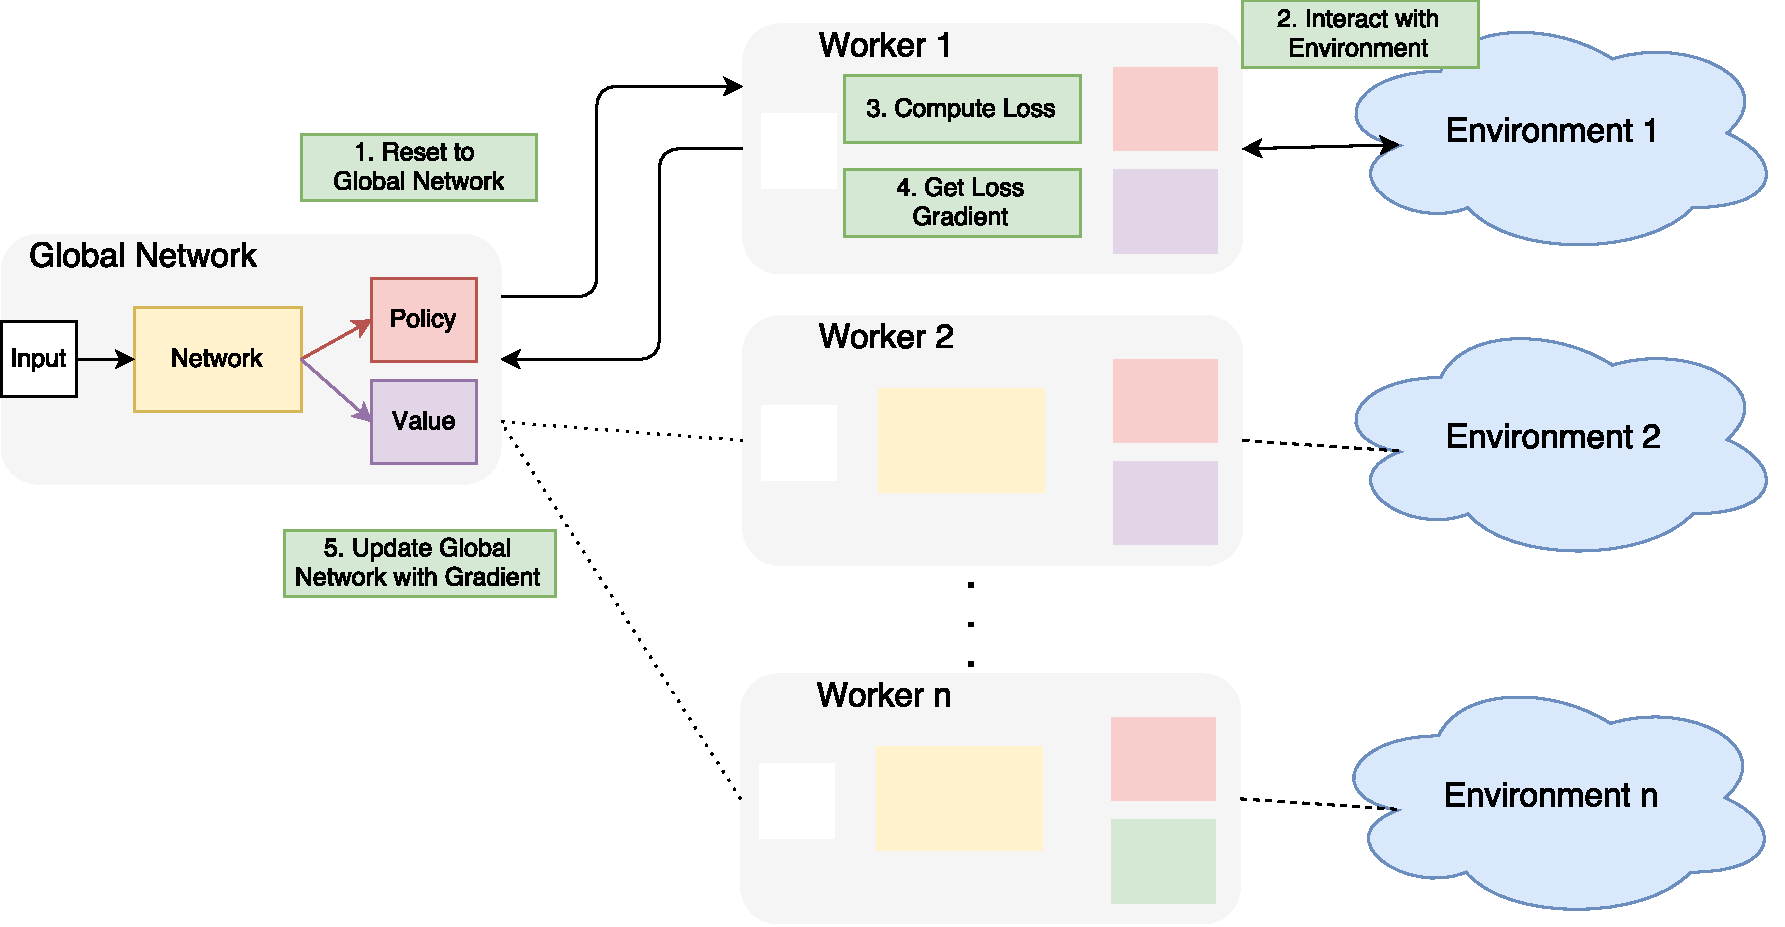
\includegraphics[width=1.25\textwidth]{Figures/Flow}
	\caption{The flow of the A3C Torcs program}
	\label{Flow}
\end{figure}
From the Figure \ref{Flow} it is possible to notice that first, a global network is defined and a number of agents or workers are instantiated to train themselves in their own environment using a copy of the global network. During training, as the first state of the environment is received and passed through all the ANN layers, the worker picks the action with the highest probability given by the output of the discrete policy layer, and then the worker executes the action while the environment returns the next state and the reward. The states keep coming during an episode and the rewards keep accumulating together with the values in an episode buffer. The episode buffer has a specific size, e.g. 100, so that after 100 episodes it becomes full, the global network is updated with the current value estimate - the bootstrap value and the episode buffer is emptied. Nevertheless, at every step, the global network is also updated with the data from the episode buffer without a bootstrap value. The update of the global network happens in a stable way thanks to the episode buffer and it is performed by applying gradients that were computed for a defined loss function.

The loss function is composed of the value loss, policy loss, and the entropy loss. The entropy loss is calculated as the logarithm of the discrete policy multiplied by the discrete policy. The value loss is calculated based on the TD error (mentioned in \ref{Temporal Difference}), which is the squared difference between the target value and the estimated value. The policy loss is computed based on the logarithm of the taken actions multiplied by their probabilities and multiplied by the advantages (mentioned earlier). Each of these is assigned specific weights in the total loss result. 

The loss function represents the performance measure, the goal, or the objective function of the current RL problem. The gradient of the loss function with respect to the weights of the ANN is calculated and applied using an optimizer. The recommended optimizers are RMSProp and, an evolved form of it - the \textit{Adaptive Moment Estimation} (Adam) optimizer. Usually, the utilized learning rate for these optimizers is 1e-4. The discount factor used in all of the calculations is 0.99.

The next chapter will present the results of training the ANN of the A3C TORCS implementation for different scenarios, including network and environment specific experiments.